\newpage
\subsection{Maze Traverse}
The job of the first agent is to traverse the maze and to generate the payload which carries all the information that has been collected by the first agent regarding the paths followed by it. The payload will then be transferred to the second robot via Bluetooth.\\
The second robot then decodes the payload and calculates the most optimal path to the destination.\\
For the purpose of maze traversal Left wall following algorithm is used.
\subsubsection{Left wall following algorithm}
This algorithm works on the basis that a maze solver will not be lost and will reach a different exit if there is any, by keeping one hand in contact will the left wall of the track. The maze solver, the first agent of the swarm in our case will always follow the left wall of the track and traverses all the tracks of the maze until it detects the target. At every junction of tracks the decision for the bots next turn is made based on which is the facing direction of the robot and determining the left side of the track. \\
The decision made by the bot on every junction is summarized in the table below:
\begin{table}[h]
\begin{center}
\begin{tabular}{ |c|c|c|c|c| } 
 \hline
 Facing & 	1 Priority & 2 priority &3 Priority&4 Priority\\ 
 \hline
 North& W &N  &E&S  \\ 
 \hline
 South & E &  S&W&N \\ 
\hline
 East&  N  & E &S & W \\
\hline
 West&S&W&N&E  \\
\hline
\end{tabular}
\caption{Decision priorities of left wall follower algorithm}
\end{center}
\end{table}
\subsubsection{Algorithm Flowchart}
\begin{figure}[h]
\center
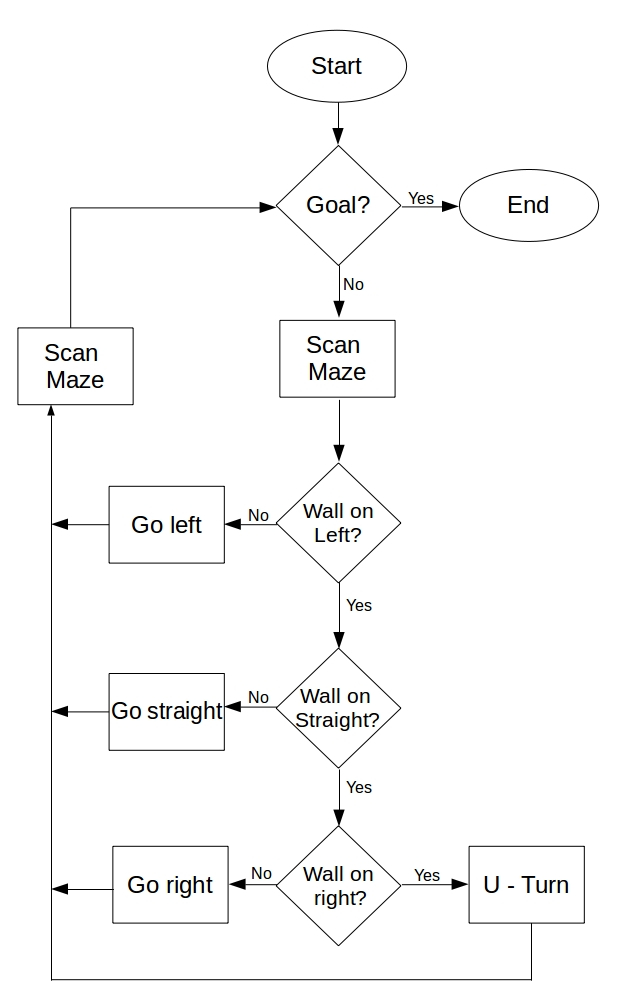
\includegraphics[scale=0.5]{flowchartnew.jpg}  
\caption{Flow-chart of left wall follower algorithm}
\end{figure}
\subsubsection{Implementation}
The leftwall following algorithm can be implemented using various models.\\ 
The model we are using contains three sensors placed at the left, right and the front facing of the robot as shown in the figure.
\begin{figure}[h]
\center
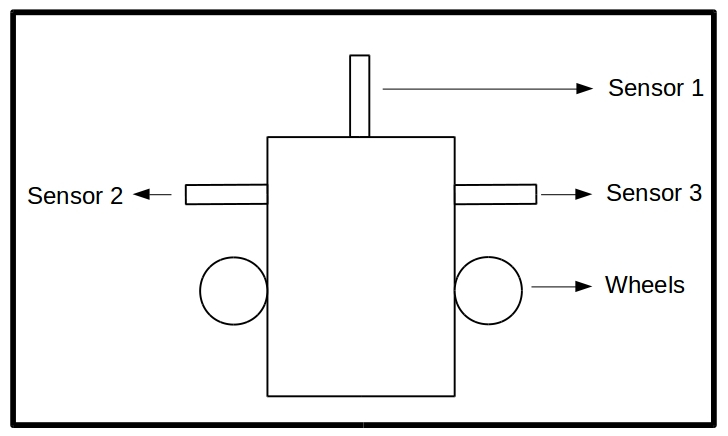
\includegraphics[scale=0.5]{bot.jpg}  
\caption{Implementation of left wall-follower algorithm}
\end{figure}
\justify The decisions are made by the robots based on the output of the all three sensors. At every junction point, which are characterized by the presence of two more than two options that the robot has to consider, the robot has to decide whether to go right or left or straight.\\
The junctions that the robot may encounter are the instants where the robot has to make the decision as to which direction to continue due to the presence of two or more options and the instants where the robot has to take a U turn. The various junctions that can be present in the maze are shown in the figure below:\begin{figure}[h]
\center
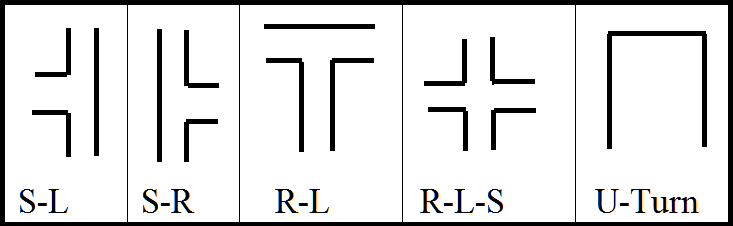
\includegraphics[scale=0.7]{Capture4.PNG} 
\caption{Possible junctions of a maze}
\end{figure}
\justify The first agent, irrespective of the position of the target always prefers the left path over straight path and straight path over the right one. The second robot however has to eliminate the mistakes made by the first robot so as to avoid reaching to the dead ends.\\
The decision made and the corresponding sensor values at the junctions are summarized in the table below:
\begin{table}[h]
\begin{center}
\begin{tabular}{ |c|c|c|c| }
\hline 
Sensor 1 (Front)&	sensor 2 (Left)	&sensor 3 (Right)&	Decision\\
\hline
High&	low	&low& 	Go left\\
\hline
Low	&low	&high&	Go left\\
\hline
Low&	high&	low	&Go straight\\
\hline
High&	high&	high&	U-turn\\
\hline
\end{tabular}
\caption{Decision made and the corresponding sensor values}
\end{center}
\end{table}
In the above table, the sensor value 'low' means there is no obstacle in the path of the sensor facing and it is clear to go whereas the sensor value 'high' means that the path faced by the sensor is blocked by the obstacles.\\
Using this algorithm the robot traverses the whole maze , through the every possible paths and reaching every junctions and the dead ends until it reaches the target, which in our case will be sensed by the smoke sensor. Further discussion on the target detection will be discussed in the later sections.\\
Now all the information gathered by the first agent about the maze structure and the decisions made at every junctions needs to be molded into the appropriate payload which can be sent through the Bluetooth module HC-05 to the second robot.\\
The discussion on how this is carried out in our project is included in the following sub-section.
\subsubsection{Payload generation}
The payload generation for the Bluetooth communication can be done by encoding the distance covered by the robot between the points of interest, but for the implementation of this model we needed an encoder.\\
Due to the unavailability of the encoders in the Nepali market and the time constraints we had, we came up with another implementation model which encodes the decision made at every junction.\\
In this implementation model, first all the junctions are assigned a number which gives the position of the junction. Then the decisions made at each junction are sent as the string of encoded binary data which are later decoded by the second robot in course of finding the most optimal path.\\
All the possible decisions which can be made at any junction are encoded using 3-bit as shown in the table below:\\
\begin{table}[h]
\begin{center}
\begin{tabular}{ |c|c| }
\hline 
Decision&	Bits\\
\hline
Left	&001\\
\hline
Straight&	010\\
\hline
Right	&011\\
\hline
U-turn	&101\\
\hline
\end{tabular}
\caption{Encoded binary values of the decisions made by the robot}
\end{center}
\end{table}
\justify The reason behind using 3-bit encoding when only four decisions can be made will be discussed in the decoding section.\\
We considered the following maze:
\newpage
\begin{figure}[h]
\center
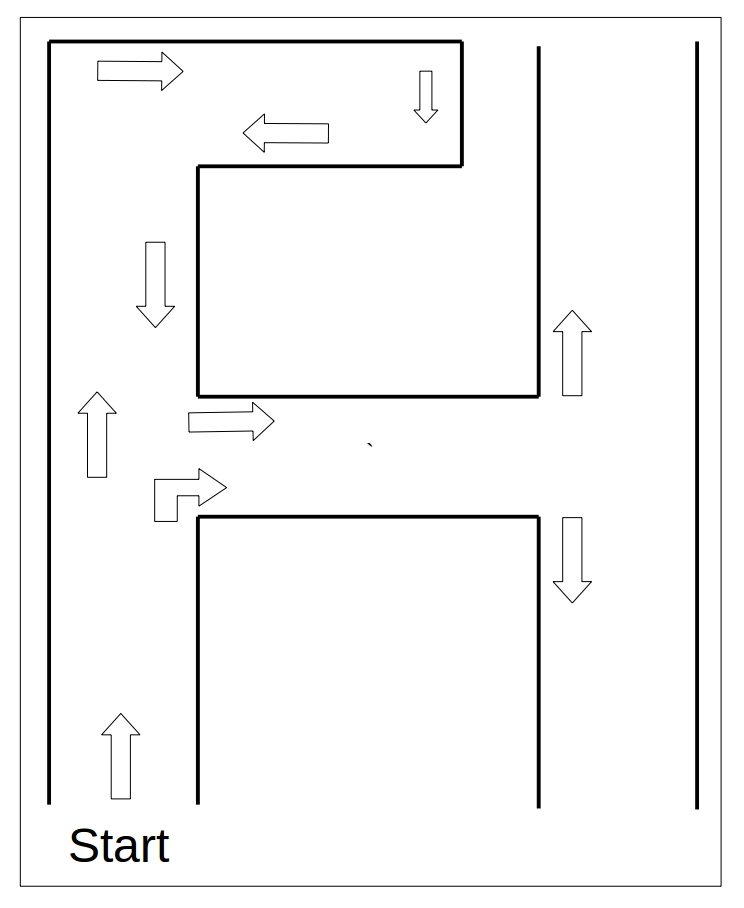
\includegraphics[scale=0.5]{mazebold.jpg}   
\caption{Example maze for illustration}
\end{figure}
\justify Now the robot starts from the starting positions and goes straight until it finds out that there are two possible paths it can continue on. At this point the first robot makes the decision based on the priorities set by the left wall following algorithm. And every decisions made by the robot is kept as the encoded binary bits in the memory.\\
In the above maze, the first robot reaches the first junction and decides to continue going straight which will then be represented as '010' and same process will be repeated until the target is reached.\\
 When the target is reached we will have a long bit string which will represent the decisions made at every junction on the group of every 3-bit of the string. The string will later be decoded by the second robot to know the decisions made by the first robot.
\subsubsection{Decoding} 
The message received by the second robot would contain a string of zeros and ones. The message encoded in this string of bits needs to be decoded to get information about the maze.\\
Let us represent the string received from the first robot as below:
\begin{table}[h]
\begin{center}
\begin{tabular}{ |c|c|c|c|c|c|c|c|c| }
\hline 
A0&	A1&	A2&	A3&	A4&	A5&	-&	-&	An\\
\hline
\end{tabular}
\caption{The representation of Bit String}
\end{center}
\end{table}
\justify A0 till An  being the individual bits of the string.\\
Each group of three bits starting from A0 would be the decision made by the first robot at the junctions  as to whether it took left, right, straight or U-turn from the junction using the encoding table previously presented.\\
The string is treated as the string of quanta of 3-bits.\\
In the case of the maze of figure ,the message sent by the first robot will be:
\begin{figure}[h]
\center
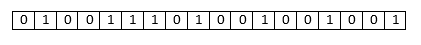
\includegraphics[scale=1]{bit.PNG}   
\caption{Received bit string for the above given maze}
\end{figure}
\justify The second robot receives first three bits and decodes that the first robot had taken straight from the first junction. Similarly it decodes the other bits and finally the decoded message sent by the first robot is shown as:
\newpage
\begin{table}[h]
\begin{center}
\begin{tabular}{ |c|c|c|c|c|c| }
\hline 
S	&R&	U&	L&	L&	L\\
\hline
\end{tabular}
\caption{The decisions made at junctions}
\end{center}
\end{table}
\justify The presence of 'U' in the message indicates that the first robot had to return to previous junction where it had taken the wrong alternative. So, every time the second robot finds 'U' in the message it eliminates the preceding bits until it encounters the junction. The junctions would be characterized by the presence of more than two options for the robot to continue.\\
If the bits  A\textsubscript{m-1} , A\textsubscript{m}, A\textsubscript{m+1} are decoded as the U-turn then the second robot eliminates the preceding bits that is  A\textsubscript{m-2},A\textsubscript{m-3},…  until it reaches the junction with more than two options i.e.  a Junction.\\ 
The reason for using 3-bits to encode just four possible decisions is, during the decoding  while the second robot has to eliminate the undesired decisions it will replace them with bits '000' so the use of 2-bit encoding would have caused problem on eliminating the undesired message bits. 
